\documentclass{article}


\usepackage{PRIMEarxiv}

\usepackage[utf8]{inputenc} % allow utf-8 input
\usepackage[T1]{fontenc}    % use 8-bit T1 fonts
\usepackage{hyperref}       % hyperlinks
\usepackage{url}            % simple URL typesetting
\usepackage{booktabs}       % professional-quality tables
\usepackage{amsfonts}       % blackboard math symbols
\usepackage{nicefrac}       % compact symbols for 1/2, etc.
\usepackage{microtype}      % microtypography
\usepackage{lipsum}
\usepackage{fancyhdr}       % header
\usepackage{float, graphicx}       % graphics
\usepackage{physics}
\usepackage{amsthm}
\pagestyle{fancy}
\thispagestyle{empty}
\rhead{ \textit{ }} 

\fancyhead[LO]{}



  

\title{\textbf{a deep dive into backtracking: solving CSPs with efficiency and accuracy}

}

\author{
  Nguyen Hoang Tan \\
  Department of Computer Science \\
  University of Information Technology \\ Linh Trung, Thu Duc\\
  \texttt{21521313@gm.uit.edu.vn} \\
}


\begin{document}
\maketitle
\theoremstyle{definition}
\newtheorem{definition}{Definition}[section]

\begin{abstract}
    Over the past twenty five years many backtracking algorithms have been developed for constraint satisfaction problems. This article describes the basic backtrack search within the search space framework and then presents a number of improvements developed in the past two decades, branching strategies, constraint propagation, nogood recording, backjumping,
    heuristics for variable and value ordering, randomization and restart strategies, and alternatives to depth-first search.
\end{abstract}

\graphicspath{Figs/}


\section{Introduction}
There are three main algorithmic techniques for solving constraint satisfaction problems:
backtracking search, local search, and dynamic programming. In this article, I survey backtracking search algorithms.\\

An algorithm for solving a constraint satisfaction problem (CSP) can be either complete
or incomplete. Complete, or systematic algorithms, come with a guarantee that a solution
will be found if one exists, and can be used to show that a CSP does not have a solution
and to find a provably optimal solution. Backtracking search algorithms and dynamic
programming algorithms are, in general, examples of complete algorithms. Incomplete, or
non-systematic algorithms, cannot be used to show a CSP does not have a solution or to
find a provably optimal solution. However, such algorithms are often effective at finding
a solution if one exists and can be used to find an approximation to an optimal solution.
Local or stochastic search algorithms are examples of incomplete algorithms. \\

Of the two classes of algorithms that are complete—backtracking search and dynamic
programming—backtracking search algorithms are currently the most important in practice. The drawbacks of dynamic programming approaches are that they often require an
exponential amount of time and space, and they do unnecessary work by finding, or making it possible to easily generate, all solutions to a CSP. However, one rarely wishes to find
all solutions to a CSP in practice. In contrast, backtracking search algorithms work on only
one solution at a time and thus need only a polynomial amount of space. \\

Since the first formal statements of backtracking algorithms over 40 years ago,
many techniques for improving the efficiency of a backtracking search algorithm have been
suggested and evaluated. In this article, I survey some of the most important techniques
including branching strategies, constraint propagation, nogood recording, backjumping,
heuristics for variable and value ordering, randomization and restart strategies, and alter-
natives to depth-first search. The techniques are not always orthogonal and sometimes
combining two or more techniques into one algorithm has a multiplicative effect (such as
combining restarts with nogood recording) and sometimes it has a degradation effect (such
as increased constraint propagation versus backjumping). Given the many possible ways
that these techniques can be combined together into one algorithm, I also survey work on
comparing backtracking algorithms. The best combinations of these techniques result in
robust backtracking algorithms that can now routinely solve large, hard instances that are of practical importance.
\section{Preliminaries}
In this section, I first define the constraint satisfaction problem followed by a brief review
of the needed background on backtracking search.
\subsection{The constraint framework}
\begin{definition}[CSP] 
    \textit{A constraint satisfaction problem (CSP) consists of a set of variables,
    $X = \{ x_1, . . . , x_n\}$; a set of values, $D = \{a_1, . . . , a_d\}$, where each variable $x_i \in X$ has an associated finite domain $dom(x_i) \subseteq D$ of possible values; and a collection of constraints.}
\end{definition}
As a running example in this survey, I will use the 6-queens problem: how can we place
6 queens on a 6 $\times$ 6 chess board so that no two queens attack each other. As one possible
CSP model, let there be a variable for each column of the board $\{x_1, . . . , x_6\}$, each with
domain $dom(x_i) = \{1, . . . , 6\}$. Assigning a value $j$ to a variable $x_i$ means placing a queen in row $j$, column $i$. Between each pair of variables $x_i$ and $x_j$ , $1 \le i < j \le 6$, there is a constraint $C(x_i, x_j )$, given by $(x_i \neq x_j ) \wedge (|i - j| \neq |x_i - x_j |)$. One possible solution is given by $\{x_1 = 4, x_2 = 1, x_3 = 5, x_4 = 2, x_5 = 6, x_6 = 3\}$. 

\subsection{Search - backtracking}
The term \textit{search} is used to represent a large category of algorithms which solve
problems by guessing an operation to perform or an action to take, possibly
with the aid of a heuristic. A good guess results in a new state
that is nearer to a goal. If the operation does not result in progress towards the
goal (which may not be apparent until later in the search), then the operation
can be retracted and another guess made.


For CSPs, search is exemplified by the backtracking algorithm. Backtracking
search uses the operation of assigning a value to a variable, so that the current
partial solution is extended. When no acceptable value can be found, the previous assignment is retracted, which is called a backtrack. In the worst case the
backtracking algorithm requires exponential time in the number of variables,
but only linear space. The algorithm was rst described more than a century
ago, and since then has been reintroduced several times.

\section{Backtracking}
A simple algorithm for solving constraint satisfaction problems is backtracking,
which traverses the search graph in a depth- first manner. The order of the
variables can be xed in advance or determined at run time. The backtracking
algorithm maintains a partial solution that denotes a state in the algorithm's
search space. Backtracking has three phases: a forward phase in which the next
variable in the ordering is selected; a phase in which the current partial solution
is extended by assigning a consistent value, if one exists, to the next variable;
and a backward phase in which, when no consistent value exists for the current
variable, focus returns to the variable prior to the current variable. 
\begin{figure}[h]
  \centering
  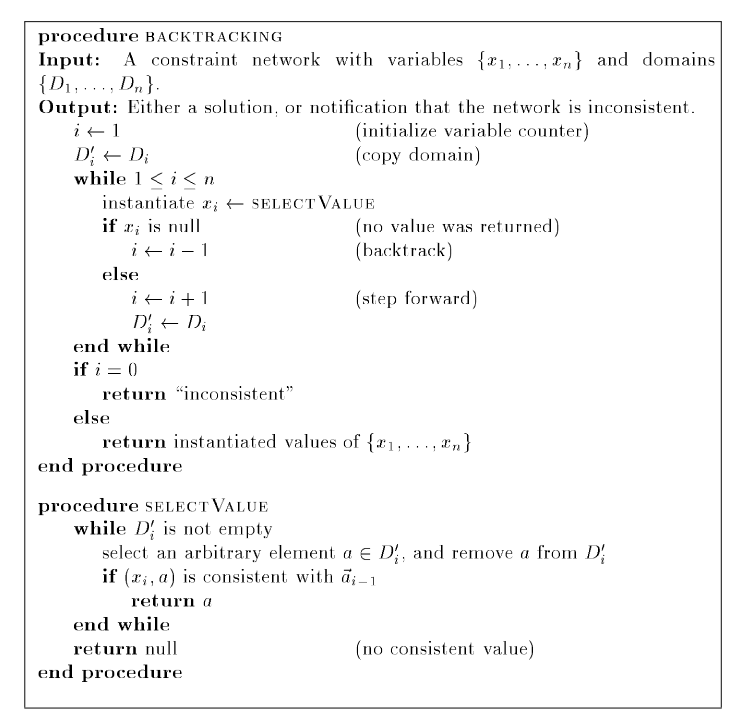
\includegraphics[scale=0.8]{Figs/backtracking-algorithm.png}
  \caption{The Backtracking algorithm}
\end{figure}
\\


Figure 1 describes a basic backtracking algorithm. As presented in Figure 1,
the backtracking algorithm returns at most a single solution, but it can easily be
modified to return all solutions, or a desired number. The algorithm employs a
series of mutable value domains \textit{$D'_i$} such that each \textit{$D'_i \in D_i. D'_i$} holds the subset of $D_i$ that has not yet been examined under the current partial instantiation.
The $D'$ sets are not needed if the values can be mapped to a contiguous set
of integers that are always considered in ascending order; in this case a single
integer can be used as a marker to divide values that have been considered from
those that have not. We use the $D'$ sets to describe backtracking for increased
generality and to be consistent with the portrayal of more complex algorithms
later in the paper. \\

The $selectValue$ subprocedure is separated from the main backtracking
routine for clarity. It has access to the current value of all variables in the main
procedure. The complexity of $selectValue$ depends on how the constraints
are represented internally. When the CSP is binary, it may be practical to store
the constraints in a table in contiguous computer memory; a one bit or one byte
flag denotes whether each possible pair of variables with corresponding values
is compatible. Accessing an entry in the table is an $O(1)$ operation. Since
the compatibility of the current candidate assignment $(x_i ; a)$ must be checked
with at most $n$ earlier variable-value pairs, the complexity of selectValue for
binary CSPs can be $O(n)$. With non-binary CSPs, checking compatibility is
more expensive for two reasons. First, the number of possible constraints is
exponential in the number of variables, and so the actual constraints are most
likely stored in a list structure. Checking the list will be $O(\log{}c)$, where $c$ is
the number of constraints. Another possibility that bears consideration is that
a constraint can be represented not as data but as a procedure. In this case the
complexity of $selectValue$ is of course dependent on the complexity of the
procedures it invokes.
\section{Improvements to backtracking}
Much of the work in constraint satisfaction during the last decade has been
devoted to improving the performance of backtracking search. Backtracking
usually suffers from thrashing, namely, rediscovering the same inconsistencies
and same partial successes during search. Efficient cures for such behavior in
all cases are unlikely, since the problem is NP-hard.

The performance of backtracking can be improved by reducing the size of
its expanded search space, which is determined both by the size of the underlying search space, and by the algorithm's control strategy. The size of the
underlying search space depends on the way the constraints are represented
(e.g. on the level of local consistency), the order of variable instantiation, and,
when one solution succes, the order in which values are assigned to each variable. Using these factors, researchers have developed procedures of two types:
those employed before performing the search, thus bounding the size of the underlying search space; and those used dynamically during the search and that
decide which parts of the search space will not be visited. Commonly used preprocessing techniques are arc- and path-consistency algorithms, and heuristic
approaches for determining the variable ordering.

The procedures for dynamically improving the pruning power of backtracking can be conveniently classified as \textit{look-ahead schemes} and \textit{look-back schemes},
in accordance with backtracking's two main phases of going forward to assemble a solution and going back in case of a dead-end. \textit{Look-ahead schemes} can
be invoked whenever the algorithm is preparing to assign a value to the next
variable. The essence of these schemes is to discover from a restricted amount
of constraint propagation how the current decisions about variable and value
selection will restrict future search. Once a certain amount of forward constraint
propagation is complete the algorithm can use the results to:
\begin{enumerate}
  \item Decide which variable to instantiate next, if the order is not predetermined. Generally, it is advantageous to first instantiate variables that maximally constrain the rest of the search space. Therefore, the most
  highly constrained variable having the least number of values, is usually selected.
  \bigskip
  \item Decide which value to assign to the next variable when there is more than
  one candidate. Generally, when searching for a single solution an attempt
  is made to assign a value that maximizes the number of options available
  for future assignments.
\end{enumerate}
\textit{Look-back schemes} are invoked when the algorithm is preparing the backtracking step after encountering a dead-end. These schemes perform two functions:
\begin{enumerate}
  \item Deciding how far to backtrack. By analyzing the reasons for the dead-end,
  irrelevant backtrack points can often be avoided so that the algorithm goes
  back directly to the source of failure, instead of just to the immediately
  preceding variable in the ordering. This procedure is often referred to as
  backjumping.
  \bigskip
  \item Recording the reasons for the dead-end in the form of new constraints, so
  that the same con icts will not arise again later in the search. The terms
  used to describe this function are constraint recording and learning.
\end{enumerate}
In sections 5 and 6 we will describe in detail several principle look-back
schemes, while section 7 will focus on look-ahead methods.
\section{Backjumping}
Backjumping schemes are one of the primary tools for reducing backtracking's
unfortunate tendency to rediscover the same dead-ends. A dead-end occurs if
$x_i$ has no consistent values left, in which case the backtracking algorithm will
go back to $x_{i-1}$. Suppose a new value for $x_{i-1}$ exists but there is no constraint
between $x_i$ and $x_{i-1}$. A dead-end will be reached at xi for each value of $x_{i-1}$ until
all values of $x{i-1}$ have been exhausted. We can finesse
this situation by identifying the \textit{culprit variable} responsible for the dead-end and
then jumping back immediately to reinstantiate the \textit{culprit variable}, instead of
repeatedly instantiating the chronologically previous variable. Identification of
a \textit{culprit variable} in backtracking is based on the notion of \textit{conflict sets}.
\begin{definition}[conflict set] 
  \textit{Let $\vec{a} = (a_1; ...; a_i)$ be a consistent instantiation,
and let $x$ be a variable not yet instantiated. If no value in the domain of $x$ is
consistent with $\vec{a}$, we say that $\vec{a}$ is a conflict set of $x$, or that $\vec{a}$ conflicts with
variable x. If, in addition, $\vec{a}$ does not contain a subtuple that is in conflict with
x, $\vec{a}$ is called a minimal conf;ict set of $x$.}
\end{definition}
\smallskip
\begin{definition}[i-leaf dead-ends] 
  \textit{Given an ordering $d = x_1;...; x_n$, then a tuple $\vec{a}_i = (a_1 ; ... a_i)$ that is consistent but is in conflict with $x_{i+1}$ is called an
  i-leaf dead-end state.}
\end{definition}
\smallskip
\begin{definition}[no-good] 
  \textit{Any partial instantiation $vec{a}$ that does not appear in
  any solution is called a no-good. Minimal no-goods have no no-good subtuples.}
\end{definition}
\smallskip
A conflict set is clearly a no-good, but there are no-goods that are not conflict
sets of any single variable. Namely, they may conflict with two or more variables.

Whenever backjumping discovers a dead-end, it tries to jump as far back
as possible without skipping potential solutions. These two issues of safety in
jumping and optimality in the magnitude of a jump need to be de ned relative
to the information status of a given algorithm. What is safe and optimal for one
style of backjumping may not be safe and optimal for another, especially if they
are engaged in different levels of information gathering.
\section{Learning Algorithms}
The earliest minimal conflict set of Definition 6.1 is a no-good explicated by
search and is used to focus backjumping. However, this same no-good may be
rediscovered again and again while the algorithm explores different paths in the
search space. By making this no-good explicit, in the form of a new constraint,
we can make sure that the algorithm will not rediscover it and, moreover, that
it may be used for pruning the search space. This technique, called \textit{constraint
recording}, is behind the learning algorithms described in this section. \\
\smallskip
\begin{definition}[earliest minimal con ict set] 
  \textit{Let $\vec{a}_i$ be a dead-end tuple whose dead-end variable is $x_{i+1}$. We denote by $emc(\vec{a}_i)$ the earliest minimal conflict set of $\vec{a}_i$ and by $par(\vec{a}_i)$ the set of variables appearing in $emc(\vec{a}_i)$. Formally, the emc is generated by selecting its members from $\vec{a}_i$ in increasing order.
  Assume that $(a_{i_1} ;...; a_{i_j} )$ were the first j members selected. Then, the first value
  appearing after $a_i$ in $\vec{a}_i$ that is inconsistent with a value of $x_{i+1}$ that was not
  ruled out by $(a_{i_1} ;...; a_{i_j} )$, will be included in emc.}
\end{definition}
By learning we mean recording potentially useful information as that information becomes known to the problem-solver during the solution process. The
information recorded is deduced from the input and involves neither generalization nor errors. An opportunity to learn (or infer) new constraints is presented
whenever the backtracking algorithm encounters a dead-end, namely, when the
current instantiation ~ai = (a1 ; :::; ai) is a con ict set of xi+1. Had the problem
included an explicit constraint prohibiting this con ict set, the dead-end would
never have been reached. The learning procedure records a new constraint that makes explicit an incompatibility that already existed implicitly in a given set
of variable assignments. There is no point, however, in recording at this stage
the conflict set $\vec{a}_i$ itself as a constraint, because under the backtracking control
strategy the current state will not recur. Yet, when $\vec{a}_i$ contains one or more
subsets that are in conflict with $x_{i+1}$ , recording these smaller conflict sets as
constraints may prove useful in the continued search; future states may contain
these conflict sets, and they exclude larger conflict sets as well. \\

With the goal of speeding up search, the target of learning is to identify
con ict sets that are as small as possible, namely, minimal. As noted above, one
obvious candidate is the earliest minimal conflict set, which is identified anyway
for conflict-directed backjumping. Alternatively, if only graph information is
used, the graph-based conflict set could be identified and recorded. Another
(extreme) option is to learn and record \textit{all} the minimal conflict sets associated
with the current dead-end. \\

In learning algorithms, the savings from possibly reducing the amount of
search by finding out earlier that a given path cannot lead to a solution must
be balanced against the costs of processing at each node generation a more
extensive database of constraints. \\

Learning algorithms may be characterized by the way they identify smaller
conflict sets. Learning can be deep or shallow. Deep learning records only the
minimal conflict sets. Shallow learning allows recording of nonminimal conflict
sets as well. Learning algorithms may also be characterized by how they bound
the arity of the constraints recorded. Constraints involving many variables are
less frequently applicable, require more space to store, and are more expensive
to consult than constraints having fewer variables. The algorithm may record a
single no-good or multiple no-goods per dead-end, and it may allow learning at
leaf dead-ends only or at internal dead-ends as well.
\section{Look-ahead Strategies}
\subsection{Combining backtracking and constraint propagation}
CSP search algorithms can combine backtracking and local constraint propagation, by applying a consistency enforcing procedure to the uninstantiated
variables. This combination is known as "looking ahead." Extending a partial
instantiation may induce constraints on the remaining variables, and making
these constraints explicit may reduce the amount of backtracking search required. Of course, actions conditioned on a partial instantiation will have to be
undone if the partial instantiation becomes no longer current due to backtracking.

While look-ahead strategies incur an extra cost after each instantiation, they
can provide several benefits. First, by removing from each future variable's domain all values that are not consistent with the partial instantiation, they eliminate the need to test values of the current variable for consistency with previous
variables. A corollary benefit is that if \textit{all} values of an uninstantiated variable
are removed by the look-ahead procedure, then the current instantiation cannot
be part of a solution and the algorithm can backtrack. Consequently, dead-ends
occur earlier in the search, and users of CSP algorithms often note much smaller
search spaces when look-ahead is employed. In general, the stronger the level
of constraint propagation, the smaller the search space explored and the higher
the computational overhead. Another benefit of look-ahead is that the sizes of
the uninstantiated variable domains can be used to guide the selection of the
variable and value to choose next.
\subsection{Look-ahead algorithms}
Look-ahead strategies that employ local consistency procedures have the same
exponential worst-case time bounds as backtracking. If the look-ahead procedure is based on arc-consistency or a weaker form of consistency, then the space
requirements are no more than maintaining the $D'$ sets. The key issue is determining experimentally a cost-effective balance between look-ahead's accuracy
and its overhead. We define four levels of look-ahead. Each employs the revise subprocedure for enforcing the arc-consistency of the constraint
between two variables.
\begin{itemize}
  \item \textit{Forward checking}. This approach, which is described in Figure 2,
  does the most limited form of constraint propagation. Forward checking
  propagates separately the effect of a tentative value selection to each of the future variables. If, as a result of calling revise the domain of one
  of these future variables becomes empty, the value is not selected and the
  next candidate value is tried.
  \begin{figure}[H]
    \centering
    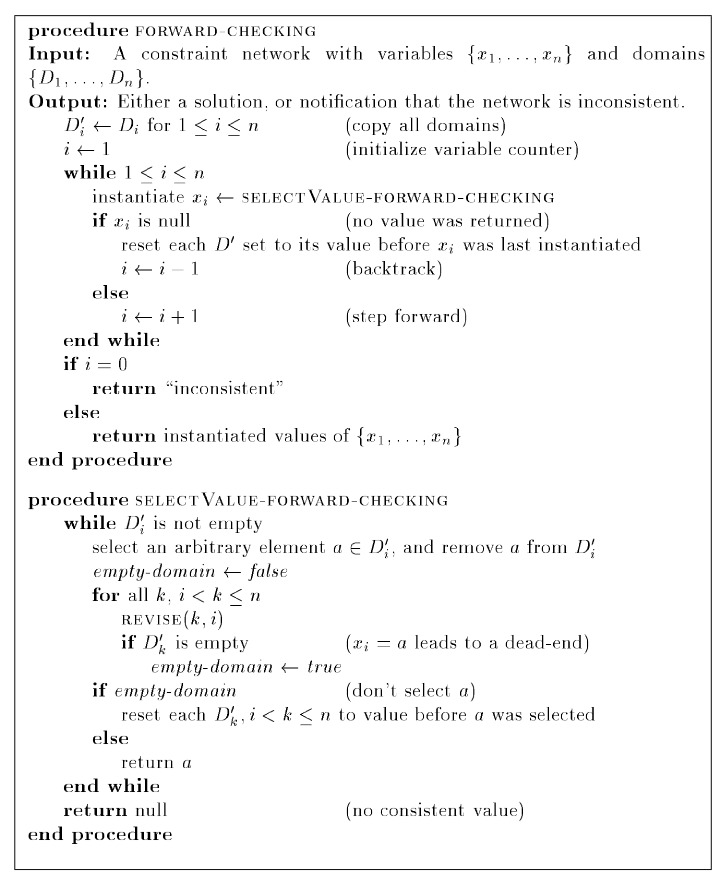
\includegraphics[scale=0.5]{Figs/forward-checking-algorithm.png}
    \caption{The forward checking algorithm}
  \end{figure}
  \item \textit{Arc-consistency look ahead}. This category includes backtracking based
  algorithms which enforce arc-consistency on the uninstantiated variables
  after each assignment of a value to the current variable. If the uninstantiated variables are not arc-consistent, namely, during the process a
  variable's domain becomes empty, then the value is rejected. Several arcconsistency enforcing algorithms have been developed; we do not specify
  which version should be used in Figure 3.
  \begin{figure}[H]
    \centering
    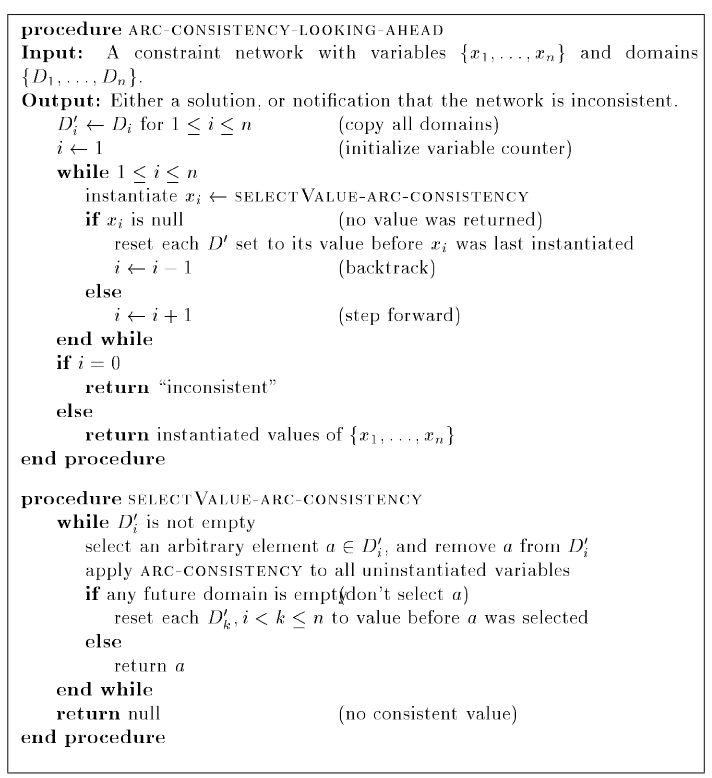
\includegraphics[scale=0.7]{Figs/arc-consistency-look-ahead.png}
    \caption{The foward checking algorithm with arc-consistency enforcing after each instantiation}
  \end{figure}
\end{itemize}
\bigskip
Our list of look-ahead techniques is not meant to be exhaustive. In particular, a search algorithm could enforce a higher degree of consistency than
arc-consistency after each instantiation. Although applying arc-consistency was
highly successful on a class of vision instances, the more extensive varieties of look-ahead have received less attention. This may be due, in part, to the negative conclusions about full looking ahead reached in: "The checks of
future with future units do not discover inconsistencies often enough to justify
the large number of tests required." More recent work has shown that as larger
and more difficult problems are experimented with, higher levels of look-ahead
become more useful.
\section{References}
\begin{enumerate}
  \item S. Arnborg. Effcient algorithms for combinatorial problems on
  graphs with bounded decomposability
  \item A. B. Baker. The hazards of fancy backtracking. In Proceedings of
  National Conference of Arti cial Intelligence.
  \item A. B. Baker. Intelligent Backtracking on constraint satisfaction problems: experimental and theoretical results. PhD thesis, Graduate
  \item Rina Dechter. Backtracking Algorithms for Constraint satisfaction problems - a tutorial survey.
  \item F. Rossi, P. van Beek. Handbook of Constraint Programing - Chapter 4: Backtracking Search Algorithms.
\end{enumerate}
\end{document}